\documentclass[12pt,a4paper,twoside,openright]{report}
\let\openright=\cleardoublepage

% Go here and change your thesis metadata!
\def\ThesisTypeTitle{Bachelor Thesis}

\def\ThesisTitle{Structuring Game Engines With Effects and Handlers}
\def\ThesisAuthor{Felix Becker}
\def\ThesisStudentID{5760770}
\def\ThesisTitlePDF{Structuring Game Engines With Effects and Handlers}
\def\ThesisAuthorPDF{Felix Becker}
\def\ThesisSubmissionDate{29.07.2025}
\def\ThesisPeriod{01.04.2025 - 31.07.2025}

\def\ThesisAbstract{
    Game engines are an essential part in the ever-growing gaming industry, as modern requirements and graphics are getting harder and harder to implement without using a game engine. The \textit{Entity Component System} architecture is a promising pattern to improve upon Object-Oriented designs in performance, flexibility, scalability and modularity through the concept of `composition over inheritance' by completely separating persistent data and behavior. Existing ECS libraries and game engines using ECS, however, are complex and implemented on a very low level.

    In this thesis, we provide a short and capable implementation of an \textit{Entity Component System} and combining it with a 2D renderer and other basic modules required for a game engine. For this, we leverage an effect system with algebraic effects and lexical handlers by using the Effekt research language. This also helps us to make the game engine as modular as possible and provide a simple and ergonomic API using just a few straightforward interfaces. We demonstrate the feasibility of the developed approach to game engines with a Snake game, serving as a case study.
}

\def\ThesisSummaryDE{
    Spiel-Engines sind ein essenzieller Teil der stetig wachsenden Spieleindustrie, da moderne Anforderungen und Grafiken immer schwerer ohne Spiel-Engines zu implementieren sind. Die \textit{Entity Component System} Architektur ist ein vielversprechendes Design Pattern um bestehende objektorientierte Designs in Performance, Flexibilität, Erweiterbarkeit und Modularität mit dem Konzept `composition over inheritance' (Komposition über Vererbung) zu verbessern, welches Daten und Verhalten (Transformation) gänzlich voneinander trennt. Bestehende ECS Bibliotheken und Spiel-Engines welche ECS verwenden sind allerdings komplex und auf eine sehr hardwarenahen Ebene implementiert.

    In dieser Arbeit zeigen wir eine kurze und fähige Implementation eines \textit{Entity Component System} und kombinieren diese mit einem 2D Renderer und anderen Basismodulen, welche für eine Spiel-Engine nötig sind. Dafür nutzen wir die Vorteile eines Effektsystems mit algebraischen Effekten und lexikalischen Handlern, welche in der Effekt Forschungssprache vorhanden sind. Dies hilft uns auch dabei, die Spiel-Engine so modular wie möglich zu machen und eine simple und ergonomische API mit nur wenigen, klaren Interfaces zu definieren. Wir demonstrieren die Nutzbarkeit des entwickelten Ansatzes für Spiel-Engines mit einem Snake Spiel, welches als Feldstudie dient.
}

\def\FirstReviewerName{Jun. Prof. Dr. Jonathan Immanuel Brachthäuser}
\def\FirstReviewerDepartment{Wilhelm-Schickard-Institut für Informatik}
\def\FirstReviewerUniversity{Universität Tübingen}

\def\Acknowledgements{
    I like to thank Ji\v{r}\'{i} Bene\v{s} and Jun. Prof. Dr. Jonathan Immanuel Brachthäuser for their support and advice during the implementation phase, as well as their feedback on writing the thesis. I also want to thank my parents for giving me the time and space to work on this thesis, as well as their support and feedback on it.
}

\def\SecondReviewerName{}


\usepackage[ngerman,english,shorthands=off]{babel}

%%% Font
\usepackage{lmodern}
\usepackage[mono=false]{libertinus}
% If you want the "classic" LaTeX feel, simply comment out the line above.

%%% Packages
% Useful "basic" packages
\usepackage{microtype}
\usepackage{amsmath,amsfonts,amsthm,bm}
\usepackage{graphicx}
\usepackage{xcolor}
\usepackage{booktabs}
\usepackage{caption}
\usepackage{floatrow}
\usepackage{array}
\usepackage{hyperref}

%%% Bibliography
\usepackage[natbib,style=numeric,sorting=none]{biblatex}
% Alternative with alphanumeric citations:
%\usepackage[natbib,style=alphabetic]{biblatex}
% Alternatives that conform to ISO690:
%\usepackage[natbib,style=iso-numeric,sorting=none]{biblatex}
%\usepackage[natbib,style=iso-alphabetic]{biblatex}

% Load bibliography entries
\addbibresource{bibliography.bib}

% TikZ (feel free to remove this if you don't need it)
\usepackage{tikz}
\usetikzlibrary{graphs,positioning} % add tikz libraries as needed

% Verbatim environments (feel free to remove this if you don't need it)
\usepackage{fancyvrb}

% Pseudocode (feel free to remove this if you don't need it)
\usepackage{algpseudocode}
\usepackage{algorithm}

% Source code (feel free to remove this if you don't need it)
\usepackage{listings}

% Type rules (feel free to remove this if you don't need it)
\usepackage{mathpartir}

% Set up PDF details
\hypersetup{pdftitle={\ThesisTitlePDF}}
\hypersetup{pdfauthor={\ThesisAuthorPDF}}
\hypersetup{unicode}
\hypersetup{breaklinks=true}

\usepackage[noabbrev]{cleveref}

% This file houses various forms of TODOs.
% You should definitely remove this file before submitting your thesis.
\usepackage[textsize=tiny, backgroundcolor=yellow!25, linecolor=black!25]{todonotes}
\newcommand{\xxx}[1]{\textcolor{red!}{#1}}
 % remove this before compiling the final version!
% use this for typesetting a chapter without a number, e.g. intro and outro
\def\chapwithtoc#1{\chapter*{#1}\addcontentsline{toc}{chapter}{#1}}

% If there is a line/figure overflowing into page margin, this will make the
% problem evident by drawing a thick black line at the overflowing spot. You
% should not disable this.
\overfullrule=3mm

% The maximum stretching of a space. Increasing this makes the text a bit more
% sloppy, but may prevent the overflows by moving words to next line.
\emergencystretch=1em

\theoremstyle{plain}
\newtheorem{theorem}{Theorem}
\newtheorem{lemma}[theorem]{Lemma}
\newtheorem{claim}[theorem]{Claim}
\newtheorem{definition}{Definition}
\theoremstyle{remark}
\newtheorem*{corrolary}{Corollary}

% real/natural numbers
\newcommand{\R}{\mathbb{R}}
\newcommand{\N}{\mathbb{N}}

% asymptotic complexity
\newcommand{\asy}[1]{\mathcal{O}(#1)}

% listings and default lstlisting config (remove if unused)
\DeclareNewFloatType{listing}{}
\floatsetup[listing]{style=ruled}

\DeclareCaptionStyle{thesis}{style=base,font={small,sf},labelfont=bf,labelsep=quad}
\captionsetup{style=thesis}
\captionsetup[algorithm]{style=thesis,singlelinecheck=off}
\captionsetup[listing]{style=thesis,singlelinecheck=off}

% Customization of algorithmic environment (comment style)
\renewcommand{\algorithmiccomment}[1]{\textcolor{black!25}{\dotfill\sffamily\itshape#1}}

% Here's how you define a custom language, Effekt is used here as an example
\lstdefinelanguage{Effekt}{
  morekeywords={%
    let,true,false,val,var,if,else,while,type,effect,interface,%
    try,with,case,do,fun,match,def,module,import,export,extern,%
    include,record,box,unbox,return,region,resource,%
    new,and,is,namespace,pure},
  otherkeywords={=>},
  alsoletter={?,!},
  sensitive=true,
  morecomment=[l]{//},
  morecomment=[n]{/*}{*/},
  morestring=[b]",
  morestring=[b]',
  morestring=[b]"""
}[keywords,comments,strings]

\floatname{listing}{Listing}
\lstset{ % use this to define styling for any other language
  language=Effekt,
  tabsize=2,
  showstringspaces=false,
  basicstyle=\footnotesize\tt\color{black!75},
  identifierstyle=\bfseries\color{black},
  commentstyle=\color{green!50!black},
  stringstyle=\color{red!50!black},
  keywordstyle=\color{blue!75!black},
  captionpos=b
}

\newcolumntype{P}[1]{>{\centering\arraybackslash}p{#1}}

\lstMakeShortInline[columns=fixed]|
 % use this file for various custom definitions

\begin{document}

% DO NOT CHANGE THIS DIRECTLY.
%
% => Change the data in `metadata.tex` instead.
%
% DO NOT CHANGE THIS DIRECTLY.

\pagestyle{empty}
\hypersetup{pageanchor=false}

\begin{titlepage}
 \begin{center}
  {\LARGE Eberhard Karls Universität Tübingen}\\
  {\large Mathematisch-Naturwissenschaftliche Fakultät \\
Wilhelm-Schickard-Institut für Informatik\\[4cm]}
  {\huge \ThesisTypeTitle\\[2cm]}
  {\Large\bf  \ThesisTitle\\[1.5cm]}
  {\large \ThesisAuthor}\\[0.5cm]
  \ThesisSubmissionDate\\[4cm]

  \ifx\SecondReviewerName\empty
    {\small\bf Reviewer}\\[1.0cm] % Note: is 0.5cm in the "original" template!
    \begin{tabular}{@{}c@{}@{}}
      {\large \FirstReviewerName{}} \\
      {\footnotesize \FirstReviewerDepartment{}} \\
      {\footnotesize \FirstReviewerUniversity{}}
    \end{tabular}
  \else
    {\small\bf Reviewers}\\[1.0cm] % Note: is 0.5cm in the "original" template!
    \begin{tabular}{@{}P{6.5cm}@{\hspace{0.5cm}}P{6.5cm}@{}}
      {\large \FirstReviewerName{}} & {\large \SecondReviewerName{}} \\
      {\footnotesize \FirstReviewerDepartment{}} & {\footnotesize \SecondReviewerDepartment{}} \\
      {\footnotesize \FirstReviewerUniversity{}} & {\footnotesize \SecondReviewerUniversity{}}
    \end{tabular}
  \fi
 \end{center}
\end{titlepage}

\vspace*{\fill}
\begin{minipage}{11.2cm}
\textbf{\ThesisAuthor:}\\
\ThesisStudentID\\
\emph{\ThesisTitle}\\
\ThesisTypeTitle\\
Eberhard Karls Universität Tübingen\\
Thesis period: \ThesisPeriod
\end{minipage}
\newpage

\hypersetup{pageanchor=true}
\pagestyle{plain}
\pagenumbering{roman}

\section*{Abstract}
\ThesisAbstract
\newpage

\section*{Zusammenfassung}
\begin{otherlanguage}{ngerman}
\ThesisSummaryDE
\end{otherlanguage}
\newpage

\section*{Acknowledgements}
\Acknowledgements
\newpage

\cleardoublepage

\ifodd\value{page}\else\newpage\fi

\tableofcontents

\cleardoublepage

\pagestyle{plain}
\pagenumbering{arabic}
\setcounter{page}{1}


\chapwithtoc{Introduction}\label{chap:introduction}

\section*{Game engines}

Game engines are used to create video games, which makes it part of a very big industry. Video games need to do massive realtime calculations on consumer hardware, which often makes game engines showcase some of the most impressive algorithms and techniques, mainly related to computer graphics. Game engines exist in various types and flavours, like smaller ones that are made for academic research or to make lightweight games as simple and straight-forward as possible to implement. Other game engines are backed by big companies and are feature-rich, tailored towards performant implementation of big and graphically advanced games.

Game engines range from simple libraries that introduce often used functions for rendering, animation, sound and more to whole frameworks that manage the complete execution flow of the game. There are even big editor programs that build a game from scripts and configuration made in a graphical user interface, which often include graphical editors for scene layout, animations, shaders, asset file management and more.

\section*{Entity Component System}

\begin{figure}
\centering
\tikzstyle{box}=[rectangle,draw,rounded corners=0.5ex,minimum height=0.5cm,minimum width=1.5cm]
\begin{tikzpicture}[thick,font=\sf\scriptsize]
\node[box,minimum height=3cm,minimum width=5cm] at (0,0) {};
\node[] at (0,1) {Archetype 1};
\node[box,fill=gray!10] at (-1.5,0.5) {Entity 1};
\node[box,fill=gray!10] at (0,0.5) {Entity 2};
\node[box,fill=gray!10] at (1.5,0.5) {Entity 3};
\node[box,fill=red!10] (a1h) at (-1.5,0) {Health};
\node[box,fill=red!10] at (0,0) {Health};
\node[box,fill=red!10] at (1.5,0) {Health};
\node[box,fill=green!10] (a1p) at (-1.5,-0.5) {Position};
\node[box,fill=green!10] at (0,-0.5) {Position};
\node[box,fill=green!10] at (1.5,-0.5) {Position};
\node[box,fill=yellow!10] (a1v) at (-1.5,-1) {Velocity};
\node[box,fill=yellow!10] at (0,-1) {Velocity};
\node[box,fill=yellow!10] at (1.5,-1) {Velocity};

\node[box,minimum height=2.5cm,minimum width=3.5cm] at (0,-3.25) {};
\node[] at (0,-2.5) {Archetype 2};
\node[box,fill=gray!10] at (-0.75,-3) {Entity 4};
\node[box,fill=gray!10] at (0.75,-3) {Entity 5};
\node[box,fill=green!10] (a2p) at (-0.75,-3.5) {Position};
\node[box,fill=green!10] at (0.75,-3.5) {Position};
\node[box,fill=yellow!10] (a2v) at (-0.75,-4) {Velocity};
\node[box,fill=yellow!10] at (0.75,-4) {Velocity};

\node[box,minimum height=2.5cm,minimum width=6.5cm] at (0,-6.25) {};
\node[] at (0,-5.5) {Archetype 3};
\node[box,fill=gray!10] at (-2.25,-6) {Entity 6};
\node[box,fill=gray!10] at (-0.75,-6) {Entity 7};
\node[box,fill=gray!10] at (0.75,-6) {Entity 8};
\node[box,fill=gray!10] at (2.25,-6) {Entity 9};
\node[box,fill=red!10] (a3h) at (-2.25,-6.5) {Health};
\node[box,fill=red!10] at (-0.75,-6.5) {Health};
\node[box,fill=red!10] at (0.75,-6.5) {Health};
\node[box,fill=red!10] at (2.25,-6.5) {Health};
\node[box,fill=green!10] (a3p) at (-2.25,-7) {Position};
\node[box,fill=green!10] at (-0.75,-7) {Position};
\node[box,fill=green!10] at (0.75,-7) {Position};
\node[box,fill=green!10] at (2.25,-7) {Position};

\node[box,align=center,fill=blue!10,minimum height=3cm,minimum width=2cm] (gs) at (-9,-1) {Move\\System};
\node[box,align=center,fill=purple!10,minimum height=3cm,minimum width=1cm] (gsq) at (-6.5,-1) {Query};
\draw[->] (gs) -- node[midway,anchor=north] {iterate} (gsq);
\draw[->] ([yshift=1cm] gsq.east) -- ([xshift=-1cm] a1p.west);
\draw[->] ([xshift=-1cm] a1p.west) -- ([xshift=0.25cm] a1p.west);
\draw[->] ([yshift=1cm] gsq.east) -- ([xshift=-1cm] a1v.west);
\draw[->] ([xshift=-1cm] a1v.west) -- ([xshift=0.25cm] a1v.west);
\draw[->] ([yshift=-1cm] gsq.east) -- ([xshift=-1cm] a2p.west);
\draw[->] ([xshift=-1cm] a2p.west) -- ([xshift=0.25cm] a2p.west);
\draw[->] ([yshift=-1cm] gsq.east) -- ([xshift=-1cm] a2v.west);
\draw[->] ([xshift=-1cm] a2v.west) -- ([xshift=0.25cm] a2v.west);

\node[box,align=center,fill=blue!10,minimum height=3cm,minimum width=2cm] (ds) at (-9,-5) {Healing\\System};
\node[box,align=center,fill=purple!10,minimum height=3cm,minimum width=1cm] (dsq) at (-6.5,-5) {Query};
\draw[->] (ds) -- node[midway,anchor=north] {iterate} (dsq);
\draw[->] ([yshift=1cm] dsq.east) -- ([xshift=-1cm] a1h.west);
\draw[->] ([xshift=-1cm] a1h.west) -- ([xshift=0.25cm] a1h.west);
\draw[->] ([yshift=-1cm] dsq.east) -- ([xshift=-1cm] a3h.west);
\draw[->] ([xshift=-1cm] a3h.west) -- ([xshift=0.25cm] a3h.west);
\end{tikzpicture}
\caption{Example ECS structure (archetype based) with 3 archetypes and 2 systems. The \textit{Move System} queries and iterates over \textit{Position} and \textit{Velocity} components, the \textit{Healing System} over \textit{Health} components.}
\label{fig:ecs}
\end{figure}

The Entity Component System concept is not a single system, but rather an architectural pattern that is often used in game engines. It is based on the principle `composition over inheritance' and therefore uses a data-oriented design instead of an object oriented design. It models a \textit{world} in terms of components, entities and systems.

\textit{Components} are a single piece of data, like a simple struct, for example a player`s/NPC character`s \textit{Health} (Integer) or \textit{Velocity} (2D or 3D Vector). \textit{Entities} are usually just an identifier or index, that identifies a single collection of these (different) components that work together to create that entity implicitly. For single instance data, like \textit{Time} or \textit{Assets}, some ECSs introduce \textit{Resources} that can be used inside a system besides component queries to hold a single value that does not belong to any entity. Other ECSs use a \textit{Singleton entity} concept for that, which ensures that such a global resource is added to one entity only.

\textit{Systems} are functions that actually transform components from one state to the next, acting on a \textit{Query} of components, independent of the purpose of the corresponding entities. These systems should not hold any data themselves, as they are only meant to define the code that transforms a set of components. Systems can then be run by the engine in their order every frame for single threaded applications. For efficient multithreading, the systems can be scheduled in parallel while avoiding any race conditions or modification during iteration. This can be done by making sure only one system has write access to a specific component type at the same time.

Many ECS libraries are \textit{archetype} based. Archetypes group entities by the set of components types they have, meaning multiple entities usually belong to the same archetype, which all have the same components with potentially different values. In the example presented in \cref{fig:ecs}, \textit{Archetype 1} could represent player entities with a |Health|, |Position| and |Velocity| component, whereas \textit{Archetype 2} with |Position| and |Velocity| could represent any simple moving object, like bullets. \textit{Archetype 3} could represent stationary enemies with just a |Health| and |Position|. The \textit{Move System} iterates all entities with |Position| and |Velocity| to modifiy the entity`s position based on its velocity. The \textit{Healing System} just iterates over all |Health| components to increase the entity`s health over time.

\section*{Effekt language}

Effekt is a research programming language developed by the Software Engineering group at the Universität Tübingen. It has an effect system and features concepts like effects, effect handlers, bidirectional effects, compile-time polymorphism, existential types and complex control flow concepts using continuations and a `program stack'. The language has so far been used mostly for smaller algorithms and systems that use the features of the language to implement them much simpler than in other languages or to showcase its features.

\textit{Effects} are like generalized exceptions. An |effect| can be defined by a single operation (function) or an |interface| that defines multiple operations which need to be implemented to handle the effect. These operations can then be called anywhere in the program, which makes the used effect get statically added as part of the type of the surrounding function. This effect then needs to be handled by an \textit{effect handler} in the surrounding code, similar to an exception handler. Only programs (`main' functions) that do not have any unhandled effects left can be executed, which can be statically checked at compile time. When an effect operation gets called, execution jumps to the closest matching handler implementation of that effect, which takes the arguments defined in the effect operation signature. Inside the implementation, the code can jump back to the original callsite by calling `resume', which calls the continuation from before the effect operation was called. The `resume' call can also return a value to the original call site, as defined by the effect operation`s signature.

\section*{TODO (problem)}

TODO

\section*{Effekt game engine}

The main contribution of this thesis is the implementation of a simple 2D game engine using the Effekt language. That involved finding ways to use Effekt`s functionality as advantages in implement a game engine based on an ECS compared to existing approaches. As a side product, it also serves as a usability test and case study of the effekt language for a larger and more complicated project. To avoid implementing low-level window creation, graphics and input, the code is compiled to the \textsf{js-web} target for now. The `foreign function interface' (\textit{ffi}) is used to interoperate with javascript functions from Effekt code. On the web target, the browser allows us to use the javascript event loop for input events and the html5 \textsf{canvas} API for simple graphics using the \textit{ffi}.

A simple but fully functional ECS builds the basis for all other engine components. Features of the Effekt language are used to make very compact code with easily comprehensible logic, but very complex control flow. This leads to an implementation of the ECS in approximately 800 lines of code, which is quite short for its rich feature set. A html5 \textsf{canvas} 2D renderer and input system are built on top of the ECS, while also using the \textit{ffi}. Once the Effekt language and general ECS concepts are understood, usage of the engine is therefore straightforward.

\section*{Structure of the Thesis}

In this thesis we discuss some existing small or research-focused game engines and compare their working principles in chapter 1, introducing the Entity Component System architecture as well. In chapter 2 we go over the Effekt language and some of its most important features for this thesis. Then we describe the implementation of our game engine and its core differences to other game engines and ECSs in chapter 3. In chapter 4 we go over details of our game engine and how I used Effekt to make it easy to use. Then we present a case study of a `Snake' game implementation in chapter 5. Afterward, we discuss some improvements, limitations and possible future work in chapter 6. In the final chapter 7, we present our conclusion of the thesis.


\chapter{Existing ECS and Game Engines}\label{chap:existing}

\section{ECS concept}

The main principle of ECS is composition over inheritance, which has many advantages not only related to performance but also flexibility, making large projects easier to expand, debug and faster to change. Performance, if optimized right, can also be much higher for large/complex scenes, as systems iterate sequentially over the required components of relevant entities. As they are mostly saved close to another, iteration is also very cache-friendly. Additionally, ECS architectures can be parallelized very easily across multiple threads, by analyzing dependencies of systems and scheduling them to avoid multiple mutable access to the same components.

A data-driven entity-based architecture with component databases for games was first implemented by the game \textsf{Thief: The Dark Project} (Looking Glass Studios, 1998). They had many financial problems during their development which shifted the focus of the game, but managed to release it working well. This was in part to their \textsf{Dark Object System}, which was the foundation for their \textsf{Dark Engine}. The system is an ECS-like database for managing all of the objects and assets in the world. It allowed game designers to modify and add/remove objects without changing code. This system worked so well, that they used it in their later game \textsf{System Shock 2} (1999), which for the most part even used the same executable of the engine.

After that, Scott Bilas from \textsf{Gas Powered Games} presented the approach they used for their \textsf{Dungueon Siege} game, with the title \textsf{A Data-Driven Game Object System} in 2002 \footnote{\url{https://www.gamedevs.org/uploads/data-driven-game-object-system.pdf}}. They needed a flexible system to manage over 7300 unique objects and over 100000 total objects in continuous, dynamically loaded maps. This should also work without engineers needing to modify and potentially hack/work around code, with the goal to empower designers to directly add objects and functionality to the world. For this problem, they also invented an object system, although it was quite different from modern ECS implementations. This presentation started to increase the attention around the ECS/data-driven architecture for games.

In 2007 Mick West from Neversoft also talked about their ECS in the article \textsf{Evolve Your Hierarchy} \footnote{\url{https://cowboyprogramming.com/2007/01/05/evolve-your-heirachy/}}. It was further popularized by Adam Martin in his extensive blogposts starting in 2007, with the title \textsf{Entity Systems are the future of MMOG development} \footnote{\url{https://t-machine.org/index.php/2007/09/03/entity-systems-are-the-future-of-mmog-development-part-1/}}. He also established most of the modern terminoligy and concepts, like systems being first-class elements that actually hold (just) their code, components holding raw data and entities being just identifiers.

\section{Existing ECS libraries}

The ECS architecture has been used in a wide range of applications, but mainly in the fields of games, simulations and other graphical/interactable media. One example is `Vico: An entity-component-system based co-simulation framework'~\cite{hatledal2021vico}. Others have improved parts of the concept, such as implementing wait-free hash maps for component access~\cite{lange2016wait}. Many more ECS libraries have been devoloped without written papers about them. Most of them are standalone for general purpose, but still intended for games and similar applications. There are so many ECS libraries in fact, that we cannot go into details comparing or grouping them, as that would be too much for the scope of this thesis. We will however go over some of the differences and data structures they use.

The first and one of the most important concepts is the memory layout of stored components. One approach is the \textit{archetype} concept, which my ECS uses as well. This means that any specific set of components an entity has at one time is called its archetype, which usually is dynamic. For dynamic approaches, any component can be added or removed from an entity at runtime, which makes it change archetypes dynamically. Examples of ECS libraries with archetypes include \textsf{flecs}\footnote{\url{https://github.com/SanderMertens/flecs}}, \textsf{decs}\footnote{\url{https://github.com/vblanco20-1/decs}}, \textsf{apecs} (by schell)\footnote{\url{https://github.com/schell/apecs}}, \textsf{hecs}\footnote{\url{https://github.com/Ralith/hecs}}, \textsf{legion}\footnote{\url{https://github.com/amethyst/legion}} and the Unity DOTS ecs package\footnote{\url{https://unity.com/ecs}}. Some of these ECS libraries combine that with a chunked approach, which splits the components of every archetype over multiple chunks, usually around 16 kB in size and memory alignment. This optimizes cache efficiency while not having to reallocate the whole array/vector when its current size limit is reached.

Another commonly used memory layout are \textit{sparse sets}, which in its core use two arrays/vectors; One is sparse and stores an index based on an item`s directly, which then points to an index in the dense array/vector where the actual data is. This dense data array/vector has no empty indices and is therefore ideal for iteration, while the sparse one is used to locate or add/remove single components. This concept is used, for example, in the ECS libraries \textsf{shipyard}\footnote{\url{https://github.com/leudz/shipyard}} and the well-known \textsf{EnTT}\footnote{\url{https://github.com/skypjack/entt}}, which is used in the game \textsf{Minecraft} (by Mojang)\footnote{\url{https://www.minecraft.net}} among others. Other ECS libraries like \textsf{bevy\textunderscore ecs}\footnote{\url{https://github.com/bevyengine/bevy/tree/main/crates/bevy_ecs}} from the \textsf{Bevy}\footnote{\url{https://bevyengine.org/}} game engine use a hybrid approach, where in this case either a simple table layout can be used for fast iteration where all components of a type are stored in a single column, or a sparse set.

Other differences between the existing ECS libraries are mostly their API with the amount of boilerplate code needed and their additional features, that go beyond the very basic and essential core of an ECS. Some require more boilerplate code to use, but can be more idiomatic for the language and potentially easier to understand and work with in large projects. Others are based on the principle to make it as easy and simple to use with the least code possible. Additional features many of the existing libraries provide include systems instead of using queries explicitly and (multithreaded) scheduling for systems. Some also have change detection to filter components that might need to be processed again, as well as relations/relationships that can build the basis for parent/child hierarchies and other relations. A few libraries also include events and triggers/observers to avoid iterating many entities when only sometimes a single event is fired that needs the entities to be processed again.

\section{ECS in existing game engines}



\section{Categorizing existing game engines}



\chapter{The Effekt language}\label{chap:effekt}

Effekt is a research-level programming language developed by the Software Engineering Group at the Universität Tübingen. It features an effect system, which provides the main features that set it apart from existing and well-known languages. Effekt can be transpiled/compiled to JavaScript, Chez Scheme or LLVM. The syntax has many similarities to Scala, which allows a very imperative programming style, while internally working on a largely functional programming model.

\section{Effects and handlers}

The main feature of Effekt are effects, which express \textit{capabilities} that are tracked with the type system \cite{brachthauser2020effects}. These capabilities can be seen as very capable exceptions for easier understanding. In most traditional languages, excaptions can be thrown and then catched in a surrounding block, which is what the simplest \textit{effect} or \textit{interface} can do. Interfaces are like effects, but they can include multiple operations together that can be handled by a single handler. `Throwing' this exception would be equivalent to calling the effect operation, like |do raise()| in effect. The `catching' (handling) looks like |try \{ ... \} with raise = \{ ... \}| then.

The effects (capabilities) that a function need from its caller and the ones it handles are included in its type signiture, so the compiler can check that all used effects are also handled \cite{brachthauser2022effects}. A |main| function can only be run if it does not have any unhandled effects. Effect handlers can also be defined via a function that takes a code block as argument (often called |prog|). Inside the handler function, the effect can be handled and the passed |prog| function called (|try \{ prog() \} with ...|). These handler functions can then be called (and in turn handle an effect) with the \textit{with} keyword, which makes the rest of the current scope`s code get passed as the first block argument. In this example it would be in the form of |with myExceptionHandler()|, where the rest of the call-site scope`s code will automatically become the |prog| argument, so afterwards |do raise()| can be called without writing the handler implementation inline and needing to indent all of the following code.

TODO: \textit{algebraic effects}

Effect operations can have argument types, which values of need to be provided in the operation call when using/calling the effect operation. In this example it could look like |do raise("We got an Error")|, meaning the effect operation argument is of the \textit{String} type.

\section{Contextual effect polymorphism}

The Effect language features lightweight contextual effect polymorphism, which means that the effects mentioned in the type signiture of a function does not need to include any effect that could potentially be used inside a computation that also gets passed to this function \cite{brachthauser2020effects}. The effects in the type signiture mention just the effects that the code of the function itself \textit{needs} to work and what it actually \textit{handles} itself. This means that a higher order function that takes another code block, for example the |map| function, can be called with a block that uses an effect (like our |raise| example). The signiture of |map| still does not mention any needed or handled effect, as it does not use the effect directly. This effect then needs to be handled at the \textit{call-site} of |map|, meaning any effect that is handled there can be used in the code block that |map| uses.

The contextual effect polymorphism describes that a \textit{pure} function is not necissarily pure, but does not use any effects itself. It can still use effects implicitly that get mentioned and handled elsewhere, like inside computations that get passed to the function.

\section{Resumtion}

Effect operations can also have a return type, which gets passed back to the call-site of the effect operation when calling the |resume| function in the handler. This gives the control flow back to where the effect operation was called \cite{brachthauser2020effects}. There, the return value of the effect operation is the value that gets passed back from the handler in the |resume| call. This makes concepts like generators and iterators possible, which are implemented in the \textit{stream} library with |read| and |emit| effects as pull and push streams. It could also pause the code execution at a point with an |await| effect and later resume there, making asynchronous programming on one thread possible.

When a handler implementation goes out of scope, it will also finish execution of all its handled effect operation calls. This means for every call of an effect operation the handler had to handle and a |resume| got called, it will continue execution after the |resume| to the end of the handler implementation. This also allows to resume multiple times, calling the continuation of the call-site of the effect operation again at a later time \cite{brachthauser2020effects}. By executing code of a handler implementation after the handler goes out of scope also allows for deferred modification and other concepts by applying the modification after the |resume| call.

\section{Bidirectional effects}

Effect operations can also use other effects themselves, which need to be handled at the call site of the effect operation. These are called bidirectional effects \cite{zhang2020bidirectional}. These are annotated as required effects in the signiture of the effect operation and their operations can be used (called) inside the handler implementation. Therefore this effect can be used in the handler without needing to be handled at the site of the handler implementation, but at the call site of the effect operation.

\section{Data types and regions}

The base data types are |String|, |Bool|,|Int|, |Double| and |Char|. These can be stored as \textit{values} (|val|, immutable) or \textit{variables} (|var|, mutable) and literals can have one of those types (e.g. "Hello", true, 3, 5.4 and 'c'). \textit{Tuples} are a way to group multiple types into a single one, surrounded by paranthesis and separated by commas. Their fields can be accessed with numbers, like |t.1|, starting from 1.

For user defined types, the simplest form is a |record|, which is like a simple struct in other languages. It can have a name (like |Vec2|) and any number of named fields. A record can just be created as a whole, there is no built-in way to assign to just a single field of a record or tuple variable. When a more complex \textit{sum}/\textit{tagged union} type is needed, a |type| can be defined instead of a record. They consist of any number of variants, which are each defined like a record.

All values and variables consisting of multiple variants or fields can also be deconstructed in a pattern \textit{match}, where each field can be assigned to a name inside the match arm directly.

The last kind of types are \textit{object}s, which are an instance of an effect (usually an interface). It is created by writing |new MyInterface \{ ... \}| instead of the typical handler with |try \{ ... \} with MyInterface \{ ... \}|. This |object| does not have fields, but all the effect operations of the respective effect can be called on it. It is a \textit{computation} type and not a \textit{value} type, which is why it is created with the |def| keyword instead of |val| or |var|. This means it cannot be returned from functions.

When an object or any other computation type, which are second-class, needs to be returned from a function, it needs to be boxed \cite{brachthauser2022effects}. Boxing a computation type makes its (potentially invisibly) captured \textit{capabilities} explicit in its type signiture. This includes \textit{region}s that specify which variables are used by the object \cite{muller2023capabilities} as well as the effects, which all need to be available in the current scope to unbox the value and use it. There are special regions for |global| and |io|, that specifies the use of the global mutable variable storage effekt uses in the background, as well as the use of input/output, like |println|.

\section{Named effect handlers}

Named effect handlers are very similar to objects, but they are not created with the |new| keyword. A named handler can be defined with a function that handles an effect or a handler directly. As seen before, handlers can be used like |with myExceptionHandler()|. When multiple handlers of the same effect are needed in the same scope simultaniously, for example to handle different kinds of exceptions with the same effect, or if it should just have a name instead of being handled for the whole sope, named effect handlers can be used \cite{xie2022named}. In this case, we could change our handler to directly take a |String| message at the call site of the handler, so it does not need to be specified for every single |raise| call.

Named effect handlers can be created using the |def| keyword similar to objects, which then looks like this: |with def outOfBounds = myExceptionHandler("Out of Bounds")|. A handler implementation can also directly name its handler like this: |try \{ ... \} with outOfBounds: raise \{ ... \}|. In both cases, the handler is now bound to the name |outOfBounds| instead of just being handled. When the |raise| operation of this effect is needed, it can now be written as |outOfBounds.raise()| instead of |do raise("Out of bounds")|. Now another exception, like |fileNotFound|, can be defined and used in the same scope.

\section{Type system and existential types}

The Effekt language has a strict type system that is enforced at compile time. This includes static type polymorphism, which is monomorphized at compile time. Another concept that is supported are existential types, which are user defined types that have a polymorphic type parameter in one or more of their variants. This type can then be the polymorphic type of fields inside the variant, for example the type of a |List[T]| field. When matching on this variant, the field can then just be used and that polymorphic type is known inside the match arm, without the actual type definition needing to annotate or keep that polymorhic type in its signiture.

This makes it possible, for example, to store (a reference to) an array with a generic type |T|, while not mentioning |T| in the signiture of that variant`s type. Therefore values containing different types of arrays can be stored in a single collection of just the plain type values. Now a function could remove any index of any of them by just needing to know the indices, but not mentioning the underlaying generic types (|T|).

\section{Namespaces and visibility}

Function, type and effect definitions can be grouped by creating namespaces, which are blocks surrounding that code. They can also be nested. To access the definitions from namespaces, its name following double colons is needed, after which the definition name can be accessed.

There are currently no visibility modifiers for definitions/fields of types, so everything of every library can always be accessed by the developer. There are multiple ways to make unwanted access of definitions clear, but they do not fully restrict the developer from using them. The most common way is having an |internal| namespace for all internal definitions. This way, the developer would have to write |...::internal::myInternalFun()|, which makes it clear this should not be used by a library user.

\chapter{Effekt ECS}\label{chap:ecs}

For our game engine library, visibility via namespaces was not feasable, as some |interface|s had internal and accessible operations, and it would be very time consuming to change this for our library. We instead chose to just prefix the internal effect operations with |internal_...|, so it would be clear as well that the developer using the library should not call these.

\section{General differences}

Comparing to existing ECS implementations, our version is an archetype based ECS and does not use chunks to store components for the same archetype. It uses effects to model all of the different parts a complete ECS needs, building up from simple ones.

The ECS uses a |Component| effect to model the component storage of all instances of a single component type. Each entity then has a (potentially different) component index for each of its components, which is not very typical for existing ECSs. Details about this system are explained in Chapter 5 (Engine implementation details and problems) in the Section `Component implementation'. This often results in non-sequential iteration of components during runtime, which is not very efficient at memory access. Although this memory inefficiency should not make a very big difference on the \textsf{js-web} target, as we discuss in more detail in Chapter 6 (Discussion).

Component queries are also implemented differently to most other ECSs. We have a |Query| effect that can be defined as a named effect handler. Inside a system, the query iteration operation on the |Query| handler can then be called, which iterates over all queried entities. Onto a |Query| handler, different components and filters can be added. When a component (including optional ones) is added to the query, a new named handler of the |CompIter| effect gets defined. Inside the |Query| iteration loop the current component from each of the |CompIter| handlers can be retrieved and modified with the respective |get| and |set| effect operations. This is explained in more detail and with examples in the Section `Queries'.

\section{World and engine}

\begin{lstlisting}[caption=Engine initialization]
with engineWorld();
with canvasRenderer();
\end{lstlisting}

To use the ECS, the |World| effect must first be handled. The engine has some additional code around the ECS that creates basic resources and systems every game needs. Using this |engineWorld| function to initialize the engine also automatically creates a |World| effect handler first. If those resources and systems should not be needed, the |world| function can be used directly. Additionally, any needed modules can be initialized/added after handling a |World| by calling their initialization functions. One of these modules is the |canvasRenderer| that is currently needed for any graphical game.

The |World| effect is used to hold all systems and run them in order. As it also represents the base structure of my ECS, the |world| function, which handles the |World| effect also handles all of the internal effects that are needed by the ECS. This includes the |ComponentManager|, |ArchManager|, |EntityIdManager|, |EntityManager| and a resource that can be toggled to exit the game loop inside of the world. Most of these are explained more thoroughly in Chapter 4 (Engine implementation details and problems). Calling the |runWorld| effect operation of the |World| effect (|do runWorld();|) starts the game loop, executing all systems in order every frame, until the escape key is pressed.

Once a |World| has been handled, any modules and game code can be added to it by creating queries and adding systems which use these queries to the |World|. Some basic resources and systems get created by the |engineWorld| function, which include |Time|, |TimeScale| and their update system. It also resets the per-frame keyboard inputs from the input module using the \textit{ffi} and exits the game loop on pressing the escape key. Other modules like the |canvasRenderer| add their components, resources and systems in a similar way. The game code by the game developer does the same as well after initialization; Creating components, resources and adding systems to the |World| using queries.

\section{Components and resources}

\begin{lstlisting}[caption=Register components example]
record Velocity(value: Vector2)
record Health(value: Int)
record EnemyTag()

def main() = {
  (...) // Init engine
  with component[Velocity]();
  with component[Health]();
  with component[EnemyTag]();
}
\end{lstlisting}

The |Component[T]| effect defines a component storage for the engine internals to store, get and set components of any single type. A handler for any type of components can be created with the |component| function. After registering, the component type can be used in all functions that need the |Component[T]| effect, for example adding it to entities.

The |Resource[T]| effect is very straightforward. When creating a resource with the |resource| function, an inital value must be provided, and that resource is then available to |get| or |set| at any time. This serves as single values that may be needed by multiple systems and should not be connected to any entity.

\section{Queries and systems}

\begin{lstlisting}[caption=Query creation example]
with def query = query();
with def velocities = query.addC[Velocity]();
with def optPositions = query.addOptC[Position]();
query.withC[Health]();
query.withoutC[EnemyTag]();
\end{lstlisting}

\textit{Queries} are used to iterate collections of specific components that can further filter which entities are included or excluded. The previous code snippet demonstrates how to create a |Query| using all its available effect operations to iterate specific components and to filter by additional ones. Handling the |Query| effect with the |query| function and binding it to a name creates an ''empty query'', meaning it will iterate over every entity without accessing any components. After that, specific (optional) components can be added to the query by calling the |addC| or |addOptC| effect operations on the previously created query. With these operations, a |CompIter| effect handler can be bound to a name, which is used during iteration of the query to |get| or |set| that component of the current entity. To filter the query additionally, the |withC| or |withoutC| effect operations can be called on the query, which will not bind any additional effect handlers. All of the |withC| components must also be present on an entity to be iterated by this query and all of the |withoutC| components must be absent. These filtered components are not iterated over; they serve only as filters to which entities get queried.

\begin{lstlisting}[caption=System example for gravity]
(..) // Create query
with system() {
  val deltaTime = (do getResource[Time]()).deltaTime;
  // Iterate query, ignoring actual "Entity" values
  query.foreach() { (_) =>
    // Update velocity
    var velocity = velocities.get().value;
    velocity = velocity + Vector2(0.0, -9.81 * deltaTime);
    velocities.set(Velocity(velocity));
    // When position exists, modify it using velocity
    positions.get() match {
      case Some(position) => positions.set(
        Some(Position(position.value + velocity * deltaTime))
      )
      case None() => ()
    };
  };
}
\end{lstlisting}

Systems are added to the |World| by calling the |system| function, which handles the |System| effect while using the |World| effect. These systems take a code block that gets called every frame, in the order the systems are added. Inside this system block, queries can be used to iterate over entities with specific components. An example of adding a system to the |World| and using our previously created query inside it to modify matching entities can be seen in the previous code snippet. This example system will apply gravity and change the position from its velocity if a position exists. This is done for every entity with |Health| that is not an enemy, which could for example match all players and allied characters, but not enemies.

\section{Entity manager}

The |EntityManager| effect gets automatically handled when using the |world| or |engineWorld|, as it is a core part of the ECS internals. It can be used to create and destroy entities and remove components from them. It can also be used to set components (or add when it is not yet present) and get the current value of components. It also has operations available to check if an entity exists or if it has a specific component. Using the |EntityManager| to create an entity returns the newly created |Entity|`s value, which can for example be stored in a component on another entity to reference it. Most of the other operations, like |setComponent| also need an |Entity| as argument, to which the operation is applied.

Inside systems, the |EntityManager| effect is overwritten by a different handler to make deferred modification possible for structural changes (create/destroy entity and add/remove components). This ensures there is no modification during iteration which could lead to an infinite loop or remove components that are yet to be iterated. Other operations, like getting a component only work if the entity already exists and immediately has the given component on it, so these are not deferred.

\chapter{Engine implementation details and problems}\label{chap:details}

\section{Component implementation}

A \textit{Component} handler creates a dynamic (resizable) array, containing all the values of that component without any empty indices. To access a component value (get or set), a component index is used. When a new component is added, it is pushed at the end of the array. Removing an index works by swapping that value with the last one and popping that last index from the array. This returns the index that was at the end before, so the surrounding/calling code can update the component index of that entity to point to the newly swapped index.

The engine internals use the component stores of each component type to store all of those values, without separating them by archetype. This way, iteration is usually not in order, but it reduces complexity and indirection. Any component value can be easily accessed by using the specific \textit{Component} effect and a component index.

When trying to destroy an entity with multiple components, a major issue occurs. Using the previously mentioned way to remove a component by using the index requires the \textit{Component} effect to be handled, which would need to be done for any component the entity currently has. As I strongly wanted dynamic entities, meaning any (single) component can be added or removed from an entity dynamically, the component types cannot be stored as part of the type of a component group. This means, the destroy entity function cannot work by using the \textit{Component} effects of all components the entity has, as that changes dynamically at runtime.

The solution for this component removal problem is using existential types and a \textit{ComponentManager}. On every component "register" using the `component' function, the \textit{ComponentManager} needs to be handled, which automatically happens when using the `world' or `engineWorld' setup functions. When a component then creates its component storage variable, it also registers it with the \textit{ComponentManager}, which gives every component type a unique index. It also stores that component storage in an array itself, wrapped in an existential type, making the type signature independed of the actual component type. When later needing to remove a component, the \textit{ComponentManager} can then be used, together with a component id and index. Inside of that remove function, the correct component storage is retrieved from an array using the id and matched on. Inside the match, that index can be removed and swapped with the last one by using the power of existential types, knowing the type of its component storage inside the removal block, without showing it in its type signature. This way, entities can be destroyed without needing to have any \textit{Component} effect handled.

\section{Archetypes and the ArchManager implementation}

The ECS needs to manage what entities have what components. As my ECS is archetype based, my \textit{ArchManager} effect takes that role. Archetypes define a specific set of component types, so every entity belongs to an archetype and many entities can and should belong to the same archetype. When a component is added or removed from an entity, its archetype changes. The \textit{ArchManager} manages these and stores which entity belongs to which archetype. It creates an archetype whenever an entity gets a component removed or added while its new archetype is not yet present and removes archetypes that no entity belongs to anymore.

My \textit{ArchManager} effect acts as the bridge between the \textit{EntityManager} and the actual component values. It has functions to check if a component type is present on a specific entity, create and destroy entities, as well as remove a component from an entity and add/set or get the value of a component. In its handler, a resizable array is created to hold all \textit{Arch} values, each representing one archetype. Each of those has a map from a component id to a resizable array, which contain all the component indices for the specific component type. Each of these is for one of the entities belonging to this archetype, in the same order as an additional resizable array in the \textit{Arch} containing all the actual \textit{Entity} values for iteration.

\section{EntityManager implementation and its API}

`Structural changes' is a term often used in ECSs to define changes that do more to the world than modify component values. They include entity creation/destruction, adding not yet present components or removing components. To summarize, `structural changes' are modifications to the world, that may lead to queries needing to recalculate their matches.

Most of the API (interaction from the game developer side) to structurally modify entities and components in the world is through the \textit{EntityManager} effect. It has functions to check if an entity exists or if it has a specific component type. It can also create and destroy entities, remove components and add/set or get component values.

The \textit{EntityManager} effect has a second handler implementation that is active inside of system bodies. They handle deferred modification, so that there is no structural modification of the queried component/entity arrays that get iterated over during modification. It forwards calls that can be executed directly to the surrounding normal \textit{EntityManager} while queuing commands that should be executed after the system, like creating entities and adding to or removing components from them. Newly created entities get reserved without yet being created, so a valid (after the system body) \textit{Entity} value can be returned that can also be used to add components to the new entity.

\section{System implementation}

A \textit{System} represents a single function or code block that gets executed once every frame of the game. When using the `system' function to add a system to the world, it creates a new \textit{System} effect handler around the currently existing one, which first calls the body of the existing system and then its own body. This way, nested \textit{System} handlers can be used to create a sequential chain of systems that get called in order or definition from the single step function the effect defines.

\section{Query implementation}



\section{World implementation and frame execution schedule}



\chapter{Case study: Snake game}\label{chap:casestudy}

The first implementation started with a simple \textit{Pong} game that was then split and evolved into the actual game engine. After most of the engine was implemented, we developed a \textit{Snake} game with and without the engine to compare both versions. In this case study, we show the differences between both versiosn and how the engine makes game development simpler and better organized.

\textit{Snake} is more of a genre than single game. The first version that was for a single player with one snake that eats apples to grow larger was \textit{Snake Byte} written by Chuck Sommerville for the Apple II and published by Sirius Software in 1982. The player can control the next direction the head of the snake turns to, which moves on a grid. \textit{Snake Byte} was based on 28 levels, whereas our version, like many simple implementations, use just a single apple. For these single level implementations, one apple always exists in the world that adds one score when eating while also increasing the snake`s length by one grid unit. The game is over when the snake head runs into an outer wall or its own tail.\\
Our version is based on this simple single level concept for the most part. A screenshot during the gameplay of this Snake implementation can be seen in \cref{fig:snake}.

\begin{figure}
\centering
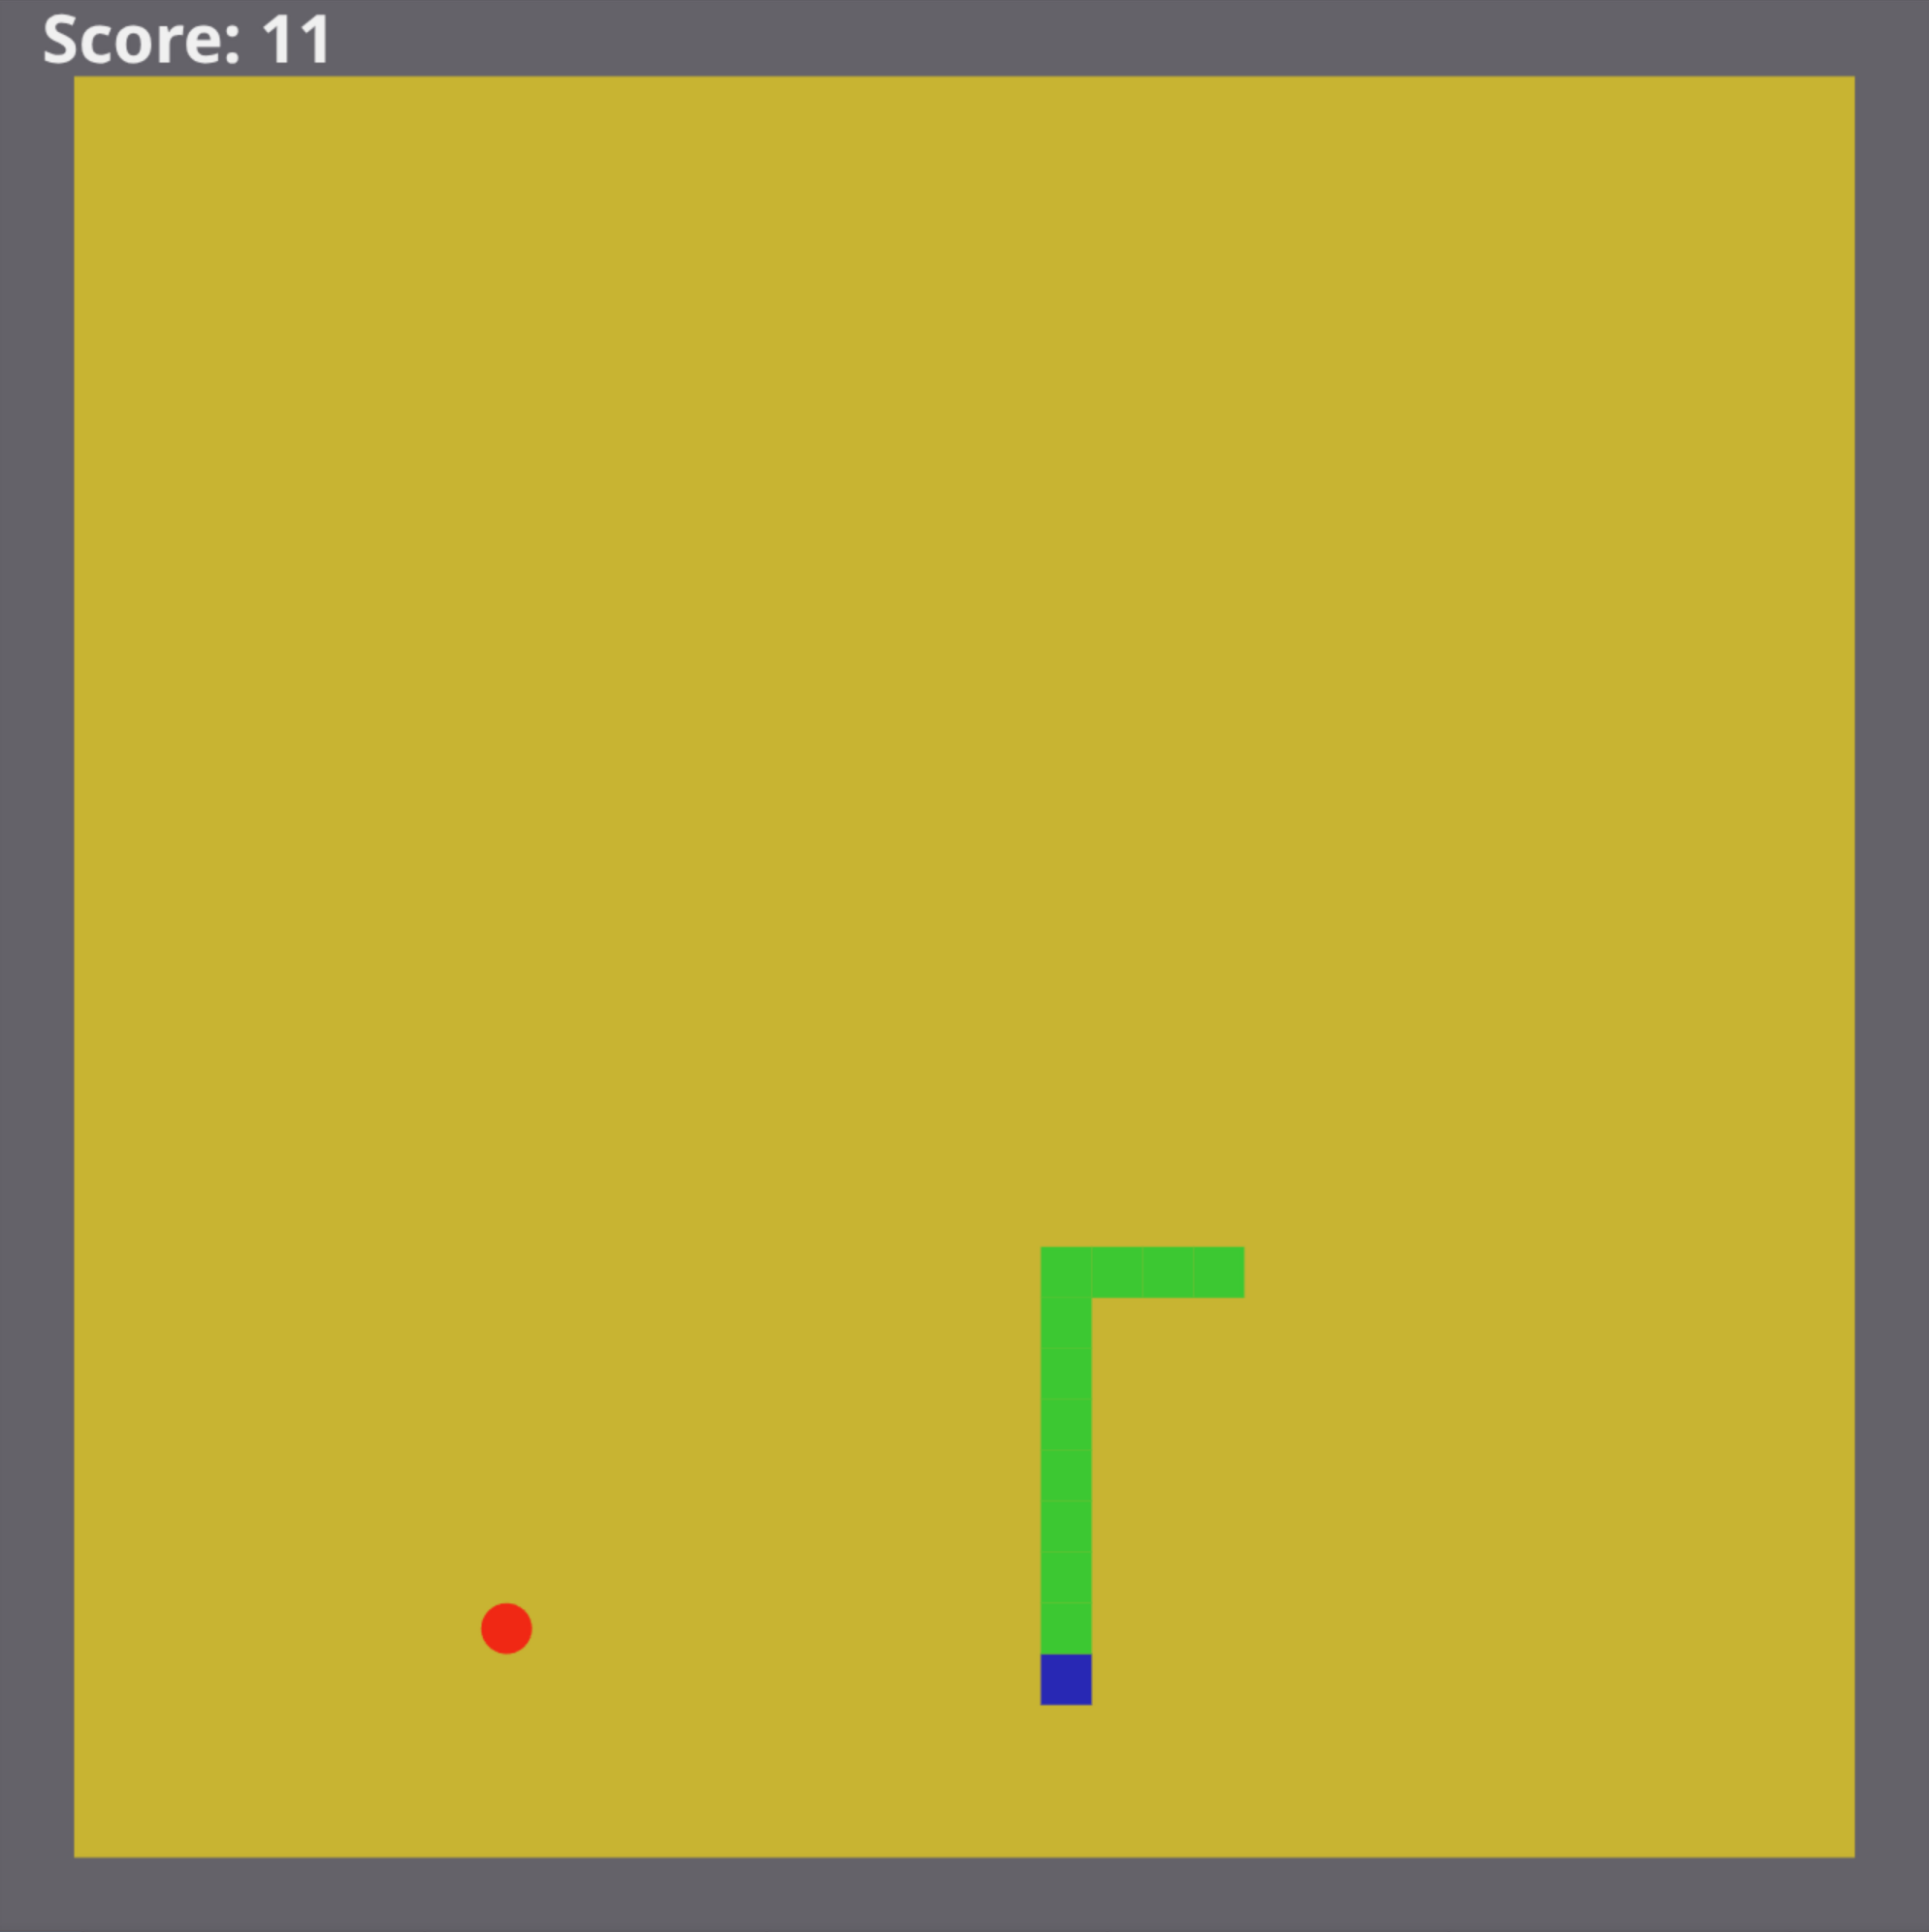
\includegraphics[width=\linewidth]{img/snake_screenshot.png}
\caption{Screenshot of the Snake Game (version using the game engine).}
\label{fig:snake}
\end{figure}

\section{Defining Components and Resources}

For the game engine version, all required components are defined as |records| at the start:

\begin{lstlisting}
record SnakeTag()
record MoveDir(next: Vector2Int, last: Vector2Int)
record LastPosition(value: Vector2)
record NextTail(value: Entity)
record Score(value: Int)
\end{lstlisting}

The components are then registered at the start of the main function after defining the default panicing ECS exception handler and initializing the |engineWorld| and |canvasRenderer|:

\begin{lstlisting}
with panicOnEcsException();

// ECS, engine & renderer init
with engineWorld();
with canvasRenderer();

// Our components
with component[SnakeTag]();
with component[MoveDir]();
...
\end{lstlisting}

The required resources are defined the same way as the components:

\begin{lstlisting}
record GameOver(value: Bool)
record MoveTimer(moveTimer: Double, doMove: Bool)
record HeadEntity(value: Entity)
record LastTailEntity(value: Entity)
record AppleEntity(value: Entity)
record ScoreEntity(value: Entity)
\end{lstlisting}

In this game, we used multiple resources to hold references to singleton entities. These have to be entities, because they represent actual visible objects in the game, so they cannot just be resources. The alternative would be to add a tag component to the entities that only the one entity has and then query on that, but using a query for a single entity is currently much less efficient than storing a reference in a resource, as any structural change makes the query need to iterate all archetypes again to find the single matching entity. These resources are then initialized after the components by providing a starting value:

\begin{lstlisting}
// Our resources
with createResource[GameOver](GameOver(false));
with createResource[MoveTimer](MoveTimer(0.0, false));
with createResource[HeadEntity](HeadEntity(invalid()));
...
\end{lstlisting}

The standalone version does not define any extra |records| to hold data, as it does not reduce the complexity or code size in this case.

\section{Initialization}

In addition to registering components and resources, the game constants are also defined at the start of the main function:

\begin{lstlisting}
// Color constants
val wallColor = Color(100, 98, 105);
val backgroundColor = Color(200, 180, 50);
...

// Game constants
val gridSize = 35;
val gridOffset = 0.5 - gridSize.toDouble() * 0.5;
val wallSize = 1.5;
val moveTime = 0.1;
val startPos = unif((gridSize / 2).toDouble());
val startDir = Vector2Int(0, 1);
val gameOverTextScale = 1.0 / 12.0;
\end{lstlisting}

These constants are defined the same way in the standalone version, but all the game state is also defined as simple variables after the constants instead of implicitly inside the entities` components.

From now on, the version with the game engine and the standalone version diverge much more, so we will just show the engine version first.

In the game engine version, the initialization of the world is defined in a local function to be able to initialize it again when restarting after a game over. This function mainly initializes resources and creates entities with the right components:

\begin{lstlisting}
def initGame() = {
  do setResource[MoveTimer](MoveTimer(moveTime, false));

  val walls = do createEntity();
  do setComponent(walls, Position(unif(0.0 - gridOffset)));
  do setComponent(
	walls, Scale(unif(gridSize.toDouble() + 2.0 * wallSize))
  );
  do setComponent(walls, Rect(wallColor));
  // Draw behind everything
  do setComponent(walls, DrawHeight(-2.0));

  ...

  val head = do createEntity();
  do setComponent(head, Position(startPos));
  ...

  do setResource[HeadEntity](HeadEntity(head));
  do setResource[LastTailEntity](LastTailEntity(head));

  var applePos: Vector2 = zero();
  each(0, gridSize * gridSize) { (_) { l } =>
    applePos = Vector2(
	  jsRandomInt(0, gridSize).toDouble(),
	  jsRandomInt(0, gridSize).toDouble()
	);
    if (startPos == applePos) {
      l.continue();
    }
    l.break();
  }

  val apple = do createEntity();
  do setComponent(apple, Position(applePos));
  do setComponent(apple, Circle(appleColor));

  ...
}
\end{lstlisting}

\section{Game Loop}

The game over state is triggered by a local function as well, which sets the |GameOver| resource as well as creating the big overlay text:

\begin{lstlisting}
def gameOver() = {
  do setResource[GameOver](GameOver(true));

  val gameOver = do createEntity();
  ...
  do setComponent(gameOver, Text(textColor, "GAME OVER"));
  ...
}
\end{lstlisting}

After this, all of the game loop is just defined by adding systems to the world and then running it with |do runWorld()|. The |initGame| function is called once before |runWorld| and then after the Enter key is pressed while in the game over state, to restart the game.

One system just updates resources and therefore does not need any queries:

\begin{lstlisting}
with system() {
  // Update game dimensions from window size
  val windowSize = (do getResource[WindowProperties]()).size;
  ...
  do setResource[Camera](Camera(
    Vector2(0.0 - gridOffset, 0.0 - gridOffset),
    0.0,
    camHeight
  ));

  // Update move timer
  if (not((do getResource[GameOver]()).value)) {
	...
    do setResource[MoveTimer](MoveTimer(moveTimer, doMove));
  }
};
\end{lstlisting}

Other systems use a query to iterate components, like the head update system, which updates the head direction based on the current key inputs:

\begin{lstlisting}
with def query = query();
with def positions = query.addC[Position]();
with def moveDirs = query.addC[MoveDir]();
query.withC[SnakeTag]();
with system() {
  if (not((do getResource[GameOver]()).value)) {
    val doMove = (do getResource[MoveTimer]()).doMove;
    query.foreach() { (_) =>
      val position = positions.get();
      val moveDir = moveDirs.get();
      var newMoveDir = moveDir.next;
      if (jsGetKeyDown("ArrowUp")
	  	&& moveDir.last.y == 0) {
        newMoveDir = Vector2Int(0, 1)
      } else if (jsGetKeyDown("ArrowDown")
	  	&& moveDir.last.y == 0) {
        newMoveDir = Vector2Int(0, -1)
      } else if (jsGetKeyDown("ArrowRight")
	  	&& moveDir.last.x == 0) {
        newMoveDir = Vector2Int(1, 0)
      } else if (jsGetKeyDown("ArrowLeft")
		&& moveDir.last.x == 0) {
        newMoveDir = Vector2Int(-1, 0)
      }
      val newLastMoveDir = if (doMove) {
        newMoveDir
      } else {
        moveDir.last
      };
      val newPosition = if (doMove) {
        Position(Vector2(
          (position.value.x.round() + newMoveDir.x).toDouble(),
          (position.value.y.round() + newMoveDir.y).toDouble()
        ))
      } else {
        position
      };
      positions.set(newPosition);
      moveDirs.set(MoveDir(newMoveDir, newLastMoveDir));
    };
  }
  ()
};
\end{lstlisting}

After these, there are systems added to update the tails based on their proceeding snake part, update the apple (find a new position), detect collisions with the head and update the score text. One system updates all the |LastPosition| components based on the |Position| components, except if a game over state occured. In this case it resets the |Position| to the |LastPosition| value, so the snake does not actually run into the object it collided with, but stops before it. One last system queries \textit{all} entities and it destroys them all when the Enter key is pressed during game over, which restarts the game, after which it calls the |initGame| function again.

\section{Differences without the game engine}

The standalone version is only slightly longer (372 versus 339 lines of code), but that version lacks some features and needed copying of significant parts of the engine code, which would need to be implemented for every single game that is not using the game engine. This includes managing the whole canvas API, dealing with window properties, direct javascript key events for input and creating its own game loop.

The first missing feature is the ability to restart the game, which would need a more complicated implementation than just a query that destroys every entity and putting the initialization code, which is needed anyway, in a local function.\\
Another feature difference is that the standalone version is always pinned to the top left corner of the available window area. The version with the game engine stays in the middle of the available window area instead of the top left, no matter if the height or width is the smaller side. This is simply a result from using the canvas renderer implementation, which uses a dynamic camera.\\
The last, missing feature is drawing circles. This means the apple is not being drawn round, but as a square as well. Drawing a circle requires multiple lines of javascript code, so it would need an additional javascript implementation in addition to the |extern| function definition in Effekt.

Other than having to copy many parts of the engine to make the standalone game work at all, the code differences include not having any vector |record|, because it would only be useful if some vector functions would be implemented along with the |record|, making the code much longer again. In the engine, vectors are implemented in the math module, including all basic math functions needed for game development. This means in the standalone version, all positions and directions are stored as separate values or variables for the X and Y value.\\
The general structure of the game loop is also much different. It defines a function to create a new apple as well es defining the whole game loop as a function. This first has to update the window properties to at least allow for dynamic resizing of the window and then updating the game time. Both of these are implemented automatically in the game engine. Then the head direction is updated directly and collision checks are done. After that the head and tail positions get updated and the head position is compared against the apple to check if it has been eaten. After all the state updates, the drawing is implemented. This part can be completely left out for the version with the game engine, as the engine does all the rendering automatically. The standalone version has to first define a function to draw a full grid rectangle based on only a grid position to make it a little bit less verbose. Then the canvas has to be cleared manually and every square that has to be drawn needs its own function call with position, size and color.

\section{Case Study Conclusion}

Regarding this case study, we conclude that the game engine abstracts and automates many details that would need to be manually implemented for every game otherwise, often also resulting in a more limiting implementation. It also structures the game in a modular way using the ECS, which is easily extensible compared to a direct approach without a game engine.\\
The size of implementation is not very different in this case, which for the most part is attributed to the ECS overhead. This is not very big, but the code size and modularity advantage would be much more obvious for a bigger and more modular game with many (dynamic) entities, as we discuss as well in the Conclusion under the Future Work section.

\chapter{Discussion}\label{chap:discussion}

\section{Unique contribution of the thesis}

After significant research, we found no real ECS based game engine, that also had an actuall implementation, in freely available academic research papers. This makes our contribution stand out, as it describes the concept and implementation of a working game engine using the ECS architecture and leveraging the Effekt language`s features.

The idea to use the ECS architecture was not present from the start, but other solutions to a generic `world'/`scene' object management system seemed hard to implement in Effekt. Considering that, the ECS architecture seemed to fit our needs and was promising to implement using effects.

\section{Restricting API usage}

Currently, the Effekt language does not provide visibility modifiers. It does offer modules, but we chose instead to prefix all function/operation names that should never be called from library user code with `internal'. Using an `internal' module would still allow the library user to call these, so modules would not be able to limit the API usage either.

Apart from calling functions/operations with the `internal' prefix, there are still other ways to use the API that are not intended. One of these is to handle multiple |World|s, registering components multiple times or handling other ECS related effects manually. This does not break the program most of the time, but can be very confusing. For example a second world would be completely separate from the first one and used until it is out of scope, but the first world will not change while a second one is handled. Registering a component for the second time will give it another type id, which will then be used until that |Component| effect is out of scope. This second handler of the component however, will not use the same storage as the first and archetypes using the second |Component| handler will be different from ones using the first.

The last major unintended API usage posibility comes from the simple fact that an effect operation can be wrapped in a local function where the effect is handled. This allows the function to not require that effect anymore, while still using the handler from the definition site directly. As explained earlier, deferred modification inside systems is made possible by handling an alternative |EntityManager| implementation (|systemEntityManager|) inside every system body to avoid infinite iteration and more. This can be circumvented by creating a function that captures the |createEntity| effect operation from outside a system using the normal |EntityManager|, but then calling that function inside a system, where it is now independent from the local deferred |EntityManager|.

The first issue can be fixed as soon as a proper system for visibility/access restriction is implemented in Effekt. The second issue of capturing an effect operation in a function can not be solved with the current concept of the Effekt language, as this builds on top of some of the core concepts of Effekt. For this, a complicated workaround would be needed to prevent this, or the library simple needs to specify that this is not allowed.

\section{Query API and drawbacks}

The initial plans for our query API was to specify the components and filters as generic types on query creation/handling and then iterate all the components via the query, not just the entity values themselfs. This turned out to not be feasable with the way the effect systems works. The current query API is quite verbose, including significant amounts of boilerplate code, but accomplishes the requirements in an easy to understand form. While easy to understand, the named handler syntax can need some getting used to.

The queries in general also are not perfect yet, as they completely recalculate their matches before the next iteration whenever any structural change was made. This means adding a component to one single entity makes all queries recalculate for the next frame. The recalculation is compromised of checking all archetypes wether they include all required components but none of the `without' filter components and creating an array for these matching archetype indices. This very conservative approach can be improved in multiple ways, as mentioned in the Conclusion, under `Future work'.

\section{Optimization and indirect component access}\label{sec:indirectaccess}

Many ECS libraries choose to store all values of a component type in separate arrays per archetype, while some even split these up into chunks of a specific size and memory alignement (often 16 kB). In both cases, many of the components that are iterated sequentially are also stored next to each other. This makes them very cache friendly and generally fast to iterate.

Our ECS uses a single dynamic array to densly store \textit{all} values of one component type and each archetype stores an additional array with indices into the component array for every entity of that archetype. This leads to one more indirection while iterating and non-sequental access of component values. While most production-ready or performance-focused ECS libraries would be significantly impacted by this, our library is for research and testing purposes. On one side, the Effekt language is not optimized for performance that much, especially the \textsf{js-web} target running on javascript. On the other side the javascript runtime with its `just in time' \textit{jit} compiler does many, often not easily predictable optimizations, which can potentially lead to this indirection not incuring any significant runtime overhead. Considering those points, having the extra indirection for component iteration should not be a relevant slowdown while making the implementation much simpler and easier to understand.

\section{Memory problems with javascript backend}

During testing of the engine and devoloping a game for a case study, we came across a problem of the current way javascript handles looping functions and the Effekt implementation.

The only way to create a continuously looping function in Effekt while giving control back to the javascript event loop to capture input events and more is to use the |wait| function, which uses the javascript |setTimeout| function. This makes the rest of the scope`s code a lambda function given to the |setTimeout|, which makes the memory allocated per-frame currently not be garbage collected. While running the case study `Snake' game, this leads to the used memory constantly increasing, crashing the game after around one minute of gameplay.

Without modifying the Effekt language, this would need a complicated workaround, which could be done in future work, as mentioned in the \cref{chap:conclusion}, under `Future work'.


\chapwithtoc{Conclusion}\label{chap:conclusion}

The goal of this thesis was to explore the advantages effect systems can have for implementing a complex game engine as well as a simple and ergonomic API. For the engine implementation, we discussed some problems in \cref{chap:discussion}, which are mostly to the Effekt language specifically. One of them is the lack of visibility modifiers in the Effekt. The other and more general problem is capturing effect operations in a local function and using that to call a handler that has a second, local, implementation that should be used instead, resulting in unintended API usage.

In general we showed that effect systems can be very helpful for designing a game engine, as it can reduce code size while simulatnuously allowing for complex control flow and maintaining readability. The ECS implementation has only about 800 lines of code, which is the main part of the engine. The effect system also allows for great modularity, making the Core Engine, Canvas Renderer and Input modules, as well as the game developer`s actual game code, easy to integrate and expand with the game engine. Some important features to make this work in Effekt are lexical effect handlers, contextual effect polymorphism, executing code after resumption, bidirectional effects, named effect handlers and existential types.

Designing a simple, straightforward and ergonomic API is also possible with effects and handlers. We showed that an API similar to established ECS libraries and game engines can be implemented with a few effect interfaces that are free to use for the game developer. These contain simple effect operations to read and modify the world, define and use components and resources, as well as create queries and systems that can be registered to run every frame. For the API, lexical effect handlers, contextual effect polymorphism, bidirectional effects and named effect handlers were also some of the most important features to achieve this.

\section*{Potential applications}

The solution presented in this thesis can be used to develop simple 2D games with Effekt. This can be the basis for future work regarding game engines, entity component systems and the Effekt language. It can also serve as a benchmark for future improvements of the Effekt language in a relatively big, complicated and performance intensive environment.

\section*{Effekt language benefits and problems}

While developing our game engine in Effekt, we came across quite a few problems, which were also in significant parts related to compiler bugs. The main reason behind this was that our game engine was one of the biggest and most complicated projects actually implemented in Effekt so far, but most of these bugs were fixed and the language generally improved during the implementation time.

After learning the concepts of Effekt and implementing a complicated project using it, we came to the conclusion that Effekt is very promising as a research language in general, while also having one of the best and easiest to use effect systems we have seen so far. It is relatively easy to learn and the effect system combined with all the concepts of the language make it very ergonomic to work with. We can recommend Effekt for future research and even small usable projects in many areas that could benefit from effect systems.

\section*{Future work}

\begin{itemize}
\item[] \textbf{LLVM port:} The current implementation uses the \textsf{js-web} target to simplify window creation, rendering backend and input by using the javascript events and canvas API. To port the game engine to LLVM, a window, input and rendering backend library compatible with LLVM would be needed. This could potentially be written (partially) in Effekt as well, or a language like C++/Rust. With this backend library, porting the game engine itself is trivial, as it uses almost no javascript specific functions apart from rendering and input handling. This could form some future research work, as that would improve performance and make it more predictable. It could then be compared to other ECS libraries, game engines and optimizations could be found and analyzed.
\item[] \textbf{Query optimization:} Queries currently update their matching archetypes once per frame if any structural changes happend in that time. This could be optimized by creating a change detection system, for example on a per-component type or per-archetype basis, so not every query would need to be updated, or not all archetypes checked on update. These ideas and more could be part of a future research work.
\item[] \textbf{Additional features:} The game engine is currently quite bare, only providing the minimum to create games much faster than without an engine while keeping a stable and extensible architecture with the ECS. Future work could expand the capabilities by adding entity hierarchies, textures/sprites, physics, making it 3D capable or other features. With an LLVM port, the possibility to use existing and capable 3D graphics or physics libraries and interfacing them with the game engine could be evaluated.
\item[] \textbf{Bigger case study game:} As mentioned in \cref{sec:memoryproblem}, even simple games do not run longer than one or two minutes becaues of a memory problem with the game loop function and the javascript backend. This only occurs for javascript, so future work could either modify Effekt or research a workaround that collects the memory of each frame. An alternative would be the LLVM port, which does not have the problem in the first place. In both cases, future work could also contain the case study of a bigger game, to better showcase the ECS advantages, as larger and more complicated games benefit more from the engine architecture. A more complicated game has not been implemented in this thesis for time reasons, as well as the memory problem.
\end{itemize}

\chapwithtoc{Bibliography}

\printbibliography[heading=none]


\appendix
\chapter{Using the Game Engine and Playing the Snake Game}

\begin{description}
\item[1. Install Effekt] as described on their website\footnote{\url{https://effekt-lang.org/docs}}.
\item[2. Clone] the Effekt 2D Game Engine repository\footnote{\url{https://github.com/airzocker/Effekt-Game-Engine-Thesis}}.
\item[3. Compile] the included \textsf{main.effekt} file with the provided \textsf{build.sh} script for Linux (Mac and Windows should work with the same command written inside the \textsf{build.sh}, but replacing \textsf{effekt.sh} with \textsf{effekt}).
\item[Or change the code] inside the \textsf{main.effekt} (it is configured to run the Snake game, using the engine, by default) and compile it
\item[Or copy] the \verb^game_engine_lib^ folder into your own project and import the required modules with \verb^import game_engine_lib/<module>^, then compile your \textsf{main.effekt}
\item[4. Open] the produced \verb^out/main.html^ file in your HTML5-capable browser
\end{description}


\openright

%%%%%%%%%%%%%%%%%%%%%%%%%%%%%%%%%%%%%%%%%%%%%%%%%%%%%%%%%%%%%%%%%%%%%%%%%%%%%
%%% Selbstständigkeitserklärung
%%%
%%% Beware: the exact wording changes often.
%%% Be sure to double-check official resources before submitting your thesis!
%%%%%%%%%%%%%%%%%%%%%%%%%%%%%%%%%%%%%%%%%%%%%%%%%%%%%%%%%%%%%%%%%%%%%%%%%%%%%
\thispagestyle{empty}
\begin{otherlanguage}{ngerman}
\section*{Selbstständigkeitserklärung}

Hiermit erkläre ich, dass ich diese schriftliche Abschlussarbeit selbständig verfasst habe, 
keine anderen als die angegebenen Hilfsmittel und Quellen benutzt habe und alle wörtlich oder sinngemäß aus anderen Werken 
übernommenen Aussagen als solche gekennzeichnet habe, 
dass die Arbeit weder vollständig noch in wesentlichen Teilen Gegenstand eines anderen Prüfungsverfahrens gewesen ist, 
dass ich die Arbeit weder vollständig noch in wesentlichen Teilen bereits veröffentlicht habe, 
dass das in Dateiform eingereichte Exemplar mit dem eingereichten gebundenen Exemplar übereinstimmt.

\vspace{1cm}
\noindent
\hrulefill \hspace{2.5cm} \hrulefill

\noindent
Ort, Datum \hfill Unterschrift
\end{otherlanguage}

\end{document}
